%
% File acl2016.tex
%
%% Based on the style files for ACL-2015, with some improvements
%%  taken from the NAACL-2016 style
%% Based on the style files for ACL-2014, which were, in turn,
%% Based on the style files for ACL-2013, which were, in turn,
%% Based on the style files for ACL-2012, which were, in turn,
%% based on the style files for ACL-2011, which were, in turn, 
%% based on the style files for ACL-2010, which were, in turn, 
%% based on the style files for ACL-IJCNLP-2009, which were, in turn,
%% based on the style files for EACL-2009 and IJCNLP-2008...

%% Based on the style files for EACL 2006 by 
%%e.agirre@ehu.es or Sergi.Balari@uab.es
%% and that of ACL 08 by Joakim Nivre and Noah Smith

\documentclass[11pt]{article}
\usepackage{acl2016}
\usepackage{times}
\usepackage{url}
\usepackage{latexsym}
\usepackage{xcolor}
\usepackage{latexsym}
\usepackage{tabularx} 
\usepackage[english]{babel}
\usepackage{multirow}
\usepackage{booktabs}
\usepackage{ifthen}
\usepackage{tikz,pgfplots}
\usepackage{xcolor,colortbl}
\usepackage[color=cyan]{todonotes}

\newcommand{\DEVELOPMENT}{1} % 1= show comments, 0=no comments
\usepackage{ifthen}
\ifthenelse{\DEVELOPMENT = 1}{
	\newcommand{\tz}[1]{\textcolor{cyan}{\textbf{TZ:} #1}}		
	\newcommand{\mw}[1]{\textcolor{red}{\textbf{MW:} #1}}				
}{
	\newcommand{\tz}[1]{}		
	\newcommand{\mw}[1]{}			
}


%\aclfinalcopy % Uncomment this line for the final submission
%\def\aclpaperid{***} %  Enter the acl Paper ID here

\setlength\titlebox{4cm}
% You can expand the titlebox if you need extra space
% to show all the authors. Please do not make the titlebox
% smaller than 5cm (the original size); we will check this
% in the camera-ready version and ask you to change it back.

\newcommand\BibTeX{B{\sc ib}\TeX}

\title{Mining Implicit Argumentation in Social Media --  \\ Status Quo}

\author{Michael Wojatzki}

\date{}

\begin{document}
\maketitle
\begin{abstract}
This status quo document has the following structure:
First, we will give a brief overview on the field of Argument Mining, outline problems we identified and state our research questions.
Second, we explain the central idea \mw{wirklich?}
Afterwards, we will show what we have done so far to examine the quality and usefulness of our model.
Finally, we will address remaining questions and problems we see in our approach and the so far conducted experiments. 
\end{abstract}



\section{Overview on State-of-the-Art and RQs}
\mw{why to deal with argmining?}
\mw{what is the sota?}
\mw{what is the performance of the sota?}
\mw{what is the problem?}
\mw{How we want to solve them? overal approach: shifting to argument perception!}

Argumentation is a constellation of propositions that is used to convince someone of a standpoint.
Especially in social media, argumentation is frequently observable and can be considered as an essential element of social media interaction such as online debates.
Since this phenomenon occurs at a massive scale, many groups of information seekers (e.g. researchers, journalists, companies, etc.) could benefit from an automated analysis of social media argumentation.
This automated identification of argumentative structures within written
communication is called argument mining \cite{green2014argmining}.
One yet unsolved problem is that --especially in informal settings -- argumentation is often done implicitly.
For instance, in a debate on atheism, one may observe an utterance such as \textit{Bible: infidels are going to hell} or even shorter \textit{\#JesusOrHell}.
In the context of a debate about atheism, both utterances implicitly express the argument that the author is against atheism, because the bible says that this will result in a stay in hell after death.
However, both claims are never explicitly mentioned.

Typically, models of argument mining assume that an argument consists of at least an explicit \textit{claim} and a number of optional supporting structures such as \textit{premises} \cite{palau2009argumentation,peldszus2013ranking}.

\mw{hier toulmin etc aufdroeseln}
\mw{performance overall, paint devastating picture here paper: "AM from info seeker perspective"}

\begin{figure*}[hbt]
\centering
  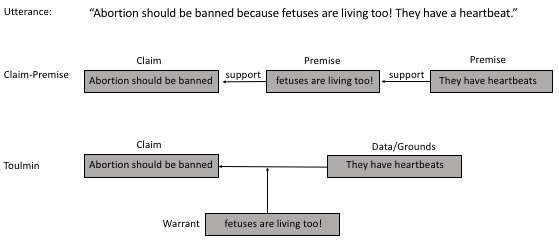
\includegraphics[width=.8\textwidth]{figures/claim_premise_toulmin.png}
  \caption{Toulmin and Freeman}
\end{figure*}


After analysing the state-of-the-art, we identified two fundamental problems of current approaches.
First, most approaches rely on strict formalisms such as the Claim-Premise-Scheme which requires that an argument is composed of exactly one claim and an arbitrarily large number of premises, justifications and other forms of support \cite{habernal2014argumentation} .
These schemes are developed to model argumentation highly elaborated, well-formed text (e.g. scientific writing or legal text) and less suited to deal with the noise and lower argument density of social media.
Second, in contrast to elaborated text, social media contains a high proportion of implicit argumentation (e.g. up to 50\% of the claims are implicit in an online debate).

In order to tackle the described problems, we propose stance-based argument mining as the topic for the dissertation.
A stance is the attitude (being in favor or against) of an author towards a given target like a politician or a controversial topic \cite{StanceSemEval2016}.
By transforming propositions into a constellation of stances towards targets, one should obtain a more abstract representation of arguments that should be more robust against implicitness and noise.
Therefore, the first milestone for the dissertation is to develop the ability detect the stance towards a defined target. 
Hence, we have already participated in the \textit{\mbox{SemEval} 2016 Task 6: Detecting Stance in Tweets} with considerable success.
As a next step, this ability should be applied to targets which are determined at runtime.
Further, experiments will be conducted which will help to model the combination of several targets into a comprehensive schema.

\section{Stance-Based Argument Mining}
\mw{also related work}
\mw{overall idea of our approach, details of first scheme in section implicit and explicit }
our approach

In order to solve the major challenge of implicit arguments that cannot be modelled well with existing approaches, we introduce a new model based on a \textit{debate stance} that will in most cases be implicit, but can be inferred from one or more \textit{explicit stances} that rely on textual evidence from the utterance.
We thereby assume that an utterance is always made in the context of a certain debate.

Figure~\ref{fig:icebergModel} gives on overview of the model which we metaphorically describe as an iceberg.
In the context of a debate about atheism, an utterance like \textit{God will judge those infidels!} is like the visible (explicit) part of the iceberg.
It expresses a stance in favor of a supernatural power (\textit{Supernatural Power}\,$\oplus$), while the actual stance on the debate target of atheism (\textit{Atheism}\,$\ominus$) is not visible but must be inferred.
Note that the debate stance might also be explicitly expressed (see figure~\ref{fig:comparison_models}a), but in implicit argumentation it has to be derived from the explicit stances.

In principle, each utterance evokes a large set of implicit stances (in a similar way as the iceberg contains a lot of invisible ice below the waterline). 
For instance, one may infer that a person uttering \textit{Bible: infidels are going to hell!} is probably in favor of praying and might have a negative stance towards issues such as abortion, same-sex marriage, etc. 
However, we argue that being in favor of Christianity already implicitly covers these stances under a common sense interpretation. 
Depending on the present informational need these targets may be more or less relevant.

An explicit stance always implicitly covers a large variety of associated stances, we propose the metaphor of an iceberg, whose actual size is also not observable but present and significant under the water surface. 

A stance which may be expressed only implicitly and may be inferred from the explicitly made stances is the second component of our model -- namely the debate stance.
This stance is important for the expressiveness of of our model, since it corresponds to the claim of other models in argument mining.

Note, that the debate stance and other stances that are implicitly covered by the explicit stances are derived as a function of the context of the present debate. 
They may be a completely different if one states the same utterance in a different debate.
For instance, in a debate on whether the Bible is judgmental book the examples in figure\ref{fig:comparison_models} would be affirmative to this target.
The two layers of the model and the iceberg metaphor are exemplified in figure~\ref{fig:icebergModel} for an utterance with one explicit stance and one utterance with two explicit stances. 


For modeling stance, we can build on plenty of research \cite{anand2011cats,somasundaran2009recognizing,sridhar2014collective,hasan2013stance} and even a shared task on automatic stance detection \cite{StanceSemEval2016}.
These works commonly define stance as being in favor of or against a given target.
Consequently, stance is a tuple consisting of a target and a stance expression such as \textit{Atheism}\,$\oplus$ or \textit{Atheism}\,$\ominus$.

Debates can be categorized in two sided debates in which authors can take a pro or contra stance and more open debates which may contain several other targets.
However, we argue that each of the targets in an open debate can be considered as a two sided debate.
Thus, if one acknowledges that the participants in a two sided debate also discuss certain sub-topics, the separation between two sided debates and open debates vanishes. 


\section{Conducted Experiments and Results}

\subsection{Automated Stance Detection}
Stance-taking is an essential and frequently observed part of online debates and other related forms of social media interaction \cite{somasundaran2009recognizing,anand2011cats}. 
In the \textit{\mbox{SemEval} 2016 Task 6: Detecting Stance in Tweets} \cite{StanceSemEval2016}, stance is defined relative to a given target like a politician or a controversial topic.
A text can then either be in favor of the given target (\textsc{Favor}), or against it (\textsc{Against}).
As the dataset also contains texts without a stance, we additionally have to deal with the the class \textsc{none}.

Being able to automatically detect and classify stance in social media is important for a deeper understanding of debates and would thus be a great tool for information seekers such as researchers, journalists, customers, users, companies, or governments.
In addition, such analysis could help to create summaries, develop a deeper understanding of online debating behavior, identify social or political groups, or even adjust recommendations to users' standpoints \cite{anand2011cats,sridhar2014collective,boltuzic2014back}.

Automated stance analysis is closely related to the task of mining arguments or sentiments \cite{boltuzic2014back}.
However, in contrast to sentiment analysis, stance is necessarily aimed at a defined target. \tz{Das ist zumindest bei aspect-oriented sentiment analysis auch so. Gibt es auch da Unterschiede?}
It is more general than argument mining, since argument mining deals with finding the reasons why someone has a certain stance or opinion \cite{boltuzic2014back}.
The aforementioned \mbox{SemEval} task represents the first shared task on stance detection that tries to explore the current state-of-the-art.
\mw{hier nochmal ins SemEval paper schauen un da die Abgrenzung herauskramen}
In the following, we describe our system for stance detection.
We did not make use of any sources of external information such as additional tweets or stance knowledge bases, as our goal was to rely only on the provided training data.
Since the task allowed just for one submission, we include some further analysis that will shed light on the usefulness and impact of the used features and parameters.

\label{sec:SubtaskA}
The goal of this subtask is to classify tweets about five targets: \textit{Atheism}, \textit{Climate Change is a Real Concern}, \textit{Feminist Movement}, \textit{Hillary Clinton}, and \textit{Legalization of Abortion}.
For each target, there are about 400-600 manually labeled tweets that can be used for training.

As the targets are quite different, we train a separate classifier for each of them. 
Additionally, we split the three-way classification into a stacked classification, in which we first classify whether the tweet contains any stance (classes \textsc{Favor} and \textsc{Against}) or no stance at all (class \textsc{None}).
In a second step, we classify the tweets labeled as containing a stance as \textsc{Favor} or \textsc{Against}.
This sequence of classifications is visualized in Figure~\ref{fig:sketch1}.

\begin{figure*}
  \centering
  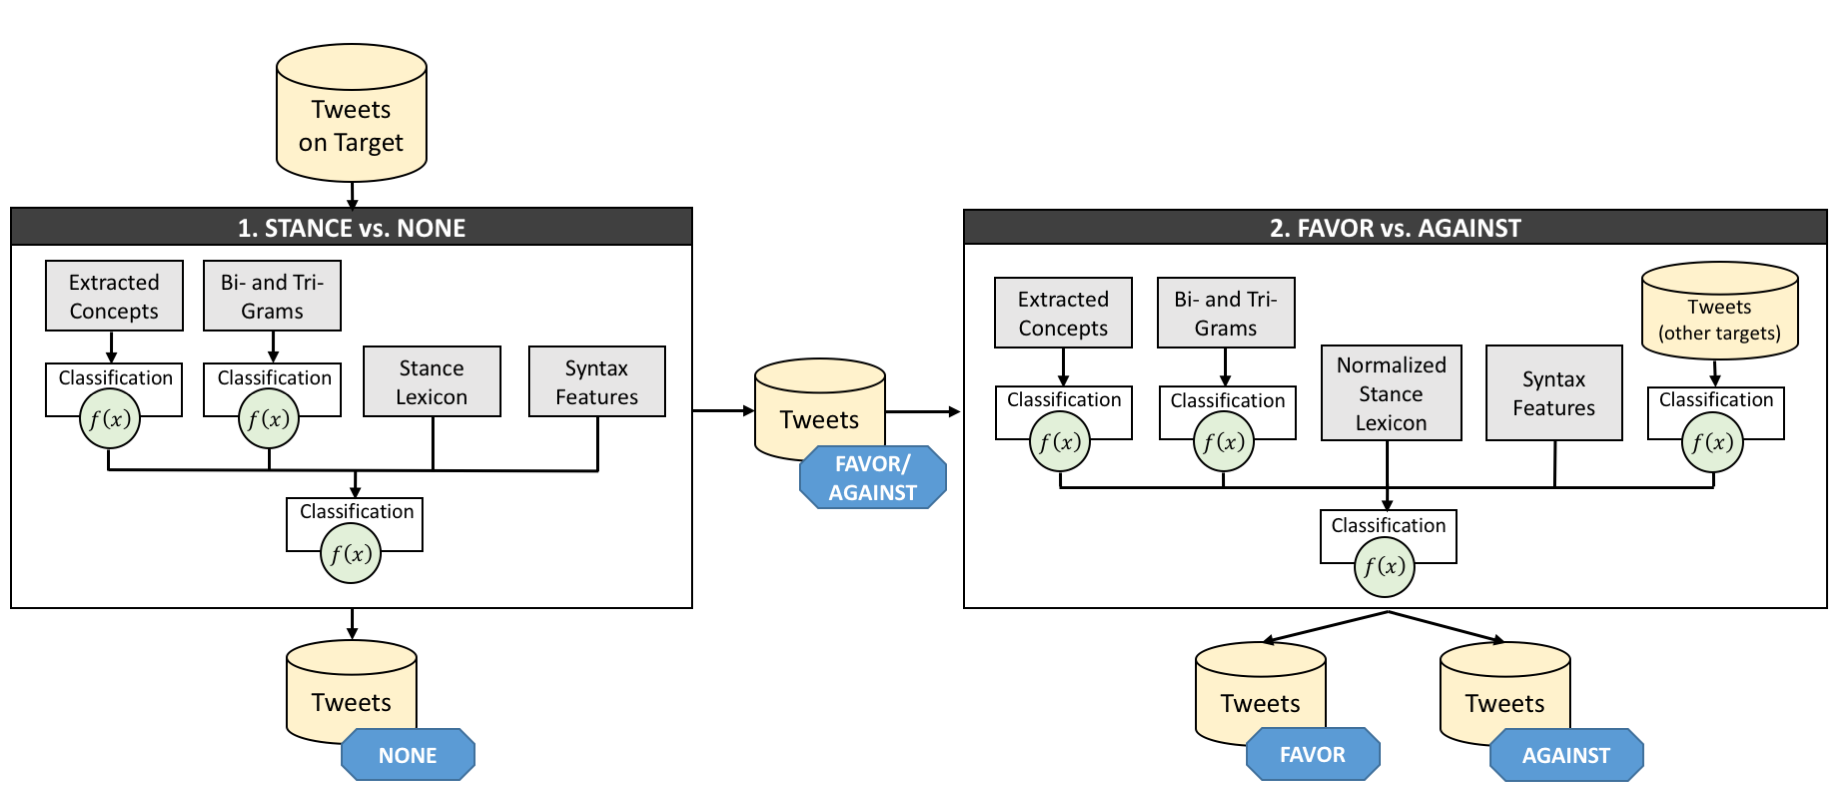
\includegraphics[scale=0.25]{figures/stance_skizze_new.png}
  \caption{Overview on the sequence of stacked classifications that is used for the supervised setting (subtask A)}
  \label{fig:sketch1}
\end{figure*}

All shown classifications are implemented using the DKPro TC framework\footnote{version 0.8.0-SNAPSHOT} \cite{daxenberger-EtAl:2014:P14-5} and utilize the integrated Weka SVM classifier.

For a detailed overview on our features and the implementation see \newcite{wojatzki2016stance}.
\mw{results}
\mw{lessons learnt}

\subsection{Explicit and Implicit Stances}
\mw{as a first step to utilize stances for a robust argumentation scheme we...}

 we utilize a semi-automated, bottom-up approach that focusses on concepts that are mostly explicitly expressed by named entities and nouns.
Consequently, we examine the frequency distributions of nouns and named entities.
Since we observe that the distribution follows Zipf's law, we expect that words with a frequency above the long tail, can serve as candidates as they occur frequently enough to avoid the sparsity problem.
It should be noted that in this corpus of Twitter messages on Atheism, the \textit{atheism} appears exactly once and the \textit{atheist} only 6 times.
This indicates that implicit argumentation is prevalent in social media.

As we want to ensure that the targets used enable us to differentiate the authors' positions sufficiently, we also consider the degree of association between nouns and named entities to the stances \textit{Atheism}\,$\oplus$ and \textit{Atheism}\,$\ominus$.
In detail, we compute the collocation coefficient $Dice$ \cite{smadja1996translating} for each word, and selected the 25 words which are most strongly associated with \textit{Atheism}\,$\ominus$ and \textit{Atheism}\,$\oplus$.

We found the resulting concepts to be too numerous and too fine-grained to be used in our model.
We thus, manually group concepts into more coarse-grained targets.
For instance, concepts such as \textit{Bible} and \textit{Jesus} are grouped into the target \textit{Christianity}.
A potential criticism of our approach is that at this stage of our work, we can not evaluate whether the set is best possible choice.
We plan to shed light on this aspect in future research. 
The final set of derived, explicit targets is shown in table~\ref{table:supportingTargets}.

\subsubsection{Annotation Process}
Using the selected data, we let three annotators identify stances towards the derived targets and the debate target.
In order to familiarize the annotators with our model, we previously trained them on a small data set that is comparable in its social media character but concerns a different target. 

Since the data partly contains utterances which cannot be understood without further context, we give annotators the option to mark them accordingly. 
Irony is another phenomenon, which influences the interpretability.
Therefore, we asked the annotators to annotate the tweets for irony as well.

Since it is still possible that our annotators interpret the tweets differently than in the original annotation, we re-annotated the debate stance using the original questionnaire described in \newcite{StanceSemEval2016}.
While annotating explicit stances, the annotators had the instruction to only annotate stances towards targets if they have textual evidence for it.
%For instance in the tweet \textit{`Whosoever abideth not in the doctrine of Christ, hath not God.' 2 John 9} we can perceive evidence for the authors standpoint for Christianity and against other religious beliefs such as Islam.
%Although is is very likely that the author is also against ideas such as \textit{secularism}, \textit{religious freedom} or that there is \textit{no evidence for religion}, we do not see textual evidence for this inference.


\subsubsection{Evaluation}
In this section, we evaluate the annotated data.
For this purpose, we first analyze the reliability of the annotation on different levels of granularity using Fleiss' Kappa ($\kappa$).
For the analysis, we exclude tweets that are annotated for irony and understandability issues.
However, we found that the annotators rarely agree on these phenomena as we get a $\kappa$ of only 0.06 for understandability and a $\kappa$ of 0.23 for irony.
Therefore, we only exclude 18 tweets in which at least two annotators share the same judgment, which results in 715 tweets for the final corpus.

\subsection{Inter Annotator Agreement}

\begin{figure*}[ht!]
\centering
\begin{tikzpicture}
        \begin{axis}[
        xbar,
            symbolic y coords={No Evidence,  Life After Death, Same-Sex Marriage, Religious Freedom, USA, Conservatism, Freethinking,no explicit target, Supernatural Power, Secularism, Islam, Christianity, , Atheism},
            ytick=data, 
            bar width= 5,
            width=.8\textwidth,
           % yticklabel style={rotate=45, anchor=east, align=center},
            height=.4\textwidth,
            xmin = 0, 
			xmax = 1,
			nodes near coords,
			enlarge y limits=0.04,
			xlabel=Fleiss' $\kappa$,
			yticklabel=\ifthenelse{\equal{\tick}{no explicit target}}{\textit{no explicit target}}{\tick}]
          ]
            \addplot[xbar,fill=blue] coordinates {
            	(0.72,Atheism)
                (0.85,Christianity)
                (0.81,Islam)
                (0.76,Secularism)
				(0.73,Supernatural Power)
                (0.73,Freethinking)
                (0.73,no explicit target)
				(0.63,Conservatism)
                (0.57,USA)
                (0.52,Religious Freedom)
				(0.51,Same-Sex Marriage)
				(0.43,Life After Death)
				(0.31,No Evidence)
            };
        \end{axis}
       % \draw [ultra thick, dashed, draw=gray](2.2,4.8)--(2.2,0); %separator (is not positioned very clever at the moment)
    \end{tikzpicture}
    \caption{Inter-annotator agreement of the debate stance \textit{Atheism} and explicit stances}
\label{fig:kappa_subTargets}
   \end{figure*}
Since the explicit targets are annotated on the basis of textual evidence, we expect a high level of agreement.
The notation of explicit targets should also result in a strong agreement of the annotation of the debate stance because it enforces a deep analysis of the communicative goal of an utterance.   
As shown in figure~\ref{fig:kappa_subTargets}, we obtain a Fleiss' $\kappa$ of 0.72 for the annotation of the debate stance.
Unfortunately, we cannot compare our agreement to the originally SemEval data, as the organizers do not report a chance corrected agreement measure for their final decision.
Also not directly comparable is the agreement of \newcite{sobhani2015argumentation} as they report weighted $\kappa$.
We argue that their weighted $\kappa$ of 0.62 is in a range similar to ours.

In figure~\ref{fig:kappa_subTargets}, we also show the agreement for the explicit targets.
Since explicit stances have a similar, deriving function like the argumentative phrases proposed by \newcite{conrad2012recognizing} and \newcite{hasan2014you}, we compare our agreements to theirs which does not exceed a Cohen's $\kappa$ of 0.68.
Two targets (\textit{Christianity} and \textit{Islam}) yield especially high agreement above $0.8$, because they are associated with clear signal words such as \textit{Jesus} and \textit{Quran} and other markers such as the numerical reference to biblical passages.
Other targets such as \textit{Secularism} and \textit{Freethinking} are rather abstract.
They hardly involve special signal words but still gain high agreements of a $\kappa$ above 0.7, which shows that our annotators did not just learn to recognize certain keywords, but can also reliably annotate more abstract targets.
This is further supported by the fact that the agreement for the annotation of \textit{no explicit target} is also in this range. 
The targets \textit{USA}, \textit{Religious Freedom}, \textit{Same-Sex Marriage}, and \textit{Life After Death} yield only a moderate agreement between 0.4 and 0.6.
An error analysis for the target \textit{Same-Sex Marriage} shows that there is disagreement if the tweet contains a stance towards gay rights in general but not to gay marriage.
We therefrom see two possibilities here to improve the agreement:
On the one hand, we could choose more comprehensive targets such as \textit{gay rights} to cover the combined positions.
On the other hand, we could train the annotators to more consistently account for such differences.
A rather low $\kappa$ of 0.31 is obtained for the target \textit{No Evidence}.
Regarding this target, we observe that annotators sometimes deviated from our guidelines and incorporated different degrees of inferred knowledge as they used \textit{Bill Nye} or \textit{Richard Dawkins}\footnote{famous supporters of the position that there is no evidence for religion} as anchors for their decisions, although the utterance contains no explicit stance in favor of \textit{No Evidence}.

Finally, we obtain a $\kappa$ of 0.63 for the joint decision on both the debate and the explicit targets.
Note that this agreement is not directly comparable with the approaches from related work, as they only implicitly model the debate stance, do not report agreements of a joint decision or rely on stances that are determined by the structure of the data.
The obtained inter-annotator agreement shows that our model can be annotated reliably and that the recognized difficulties may be compensated by a better training of the annotators and a better selection of targets.
   
\subsubsection{Stance Pattern Analysis}

\begin{figure}[ht!]
\centering
  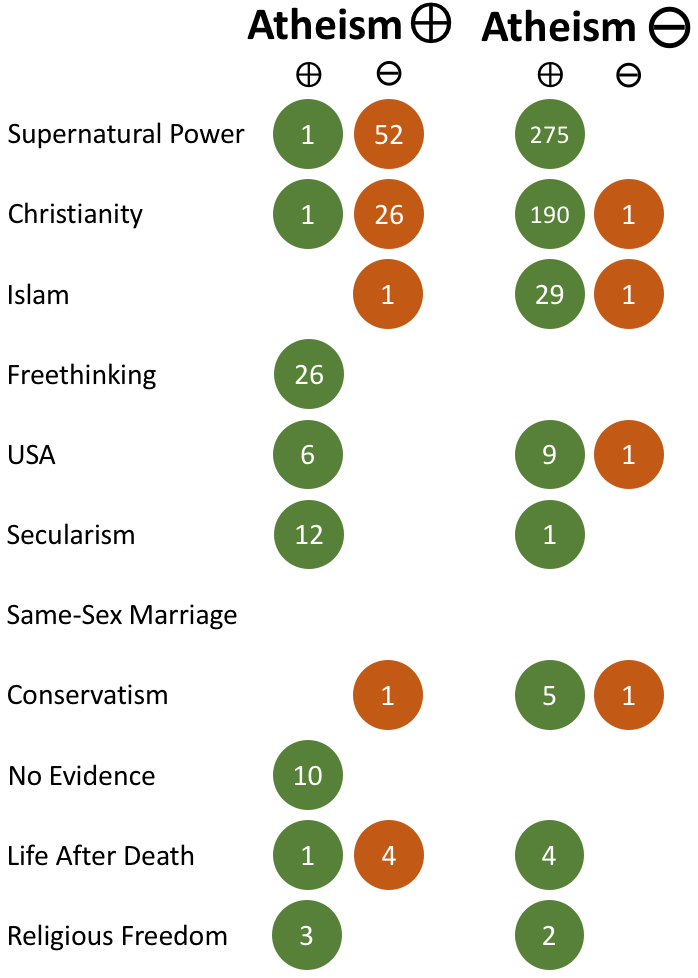
\includegraphics[width=0.45\textwidth]{figures/patterns_flat.png}
  \caption{Frequency of explicit stances grouped according to debate stance}
  \label{fig:patterns_flat}
\end{figure}

In order to inspect usage patterns of explicit stance taking, we must agree on one annotation for each tweet.
Since we do not assume that there are differences in the quality of the three annotators, we rely on a majority vote to compile a final annotation. 

Figure~\ref{fig:patterns_flat} visualizes the frequency of the explicitly taken stances for Atheism\,$\oplus$ and Atheism\,$\ominus$.
It shows that there are significant differences in the argumentation patterns between the two camps.
As expected, if advocates of atheism are against a target such as \textit{Christianity}, the opponents are mostly in favor of it or do not mention it.
This pattern is also observable for the reverse case such as for \textit{Freethinking}.
Note that utterances addressing the target \textit{Same-Sex Marriage} are exclusively annotated for expressing no stance towards \textit{Atheism}.
Further exceptions are the targets \textit{USA} and \textit{Religious Freedom} that are positively mentioned by both camps.
However, a deeper analysis shows that these targets always occur together with other targets which seem to be more relevant for the debate stance.

In order to analyze stance patterns in more details, we show which other stances are used together with the target \textit{Supernatural Power} (the most frequent target in both camps) in figure~\ref{fig:patterns_combined}.
We observe that authors that are in against Atheism use \textit{Christianity}\,$\oplus$ together with \textit{Supernatural Power}\,$\oplus$ in 50\% of all cases.
In contrast, authors that are in favor of Atheism only combine \textit{Supernatural Power}\,$\ominus$ with \textit{Christianity}\,$\ominus$ in 13\% of all cases.
The figure also shows that the other explicit stances only play a subordinate role in the combination with those targets.

%The results can be interpreted to mean that a majority of the authors being against atheism comment on the subject by expressing their belief in an supernatural being or Christianity.
%At the same time, the advocates of atheism express their disbelieves in those targets.
From these analyses we can conclude that stable patterns of argumentation using explicit stances other than the debate stance exist.
This is a strong indication for the validity of our assumption that the debate stance can be inferred from explicitly expressed stances.


\begin{figure*}
\centering
  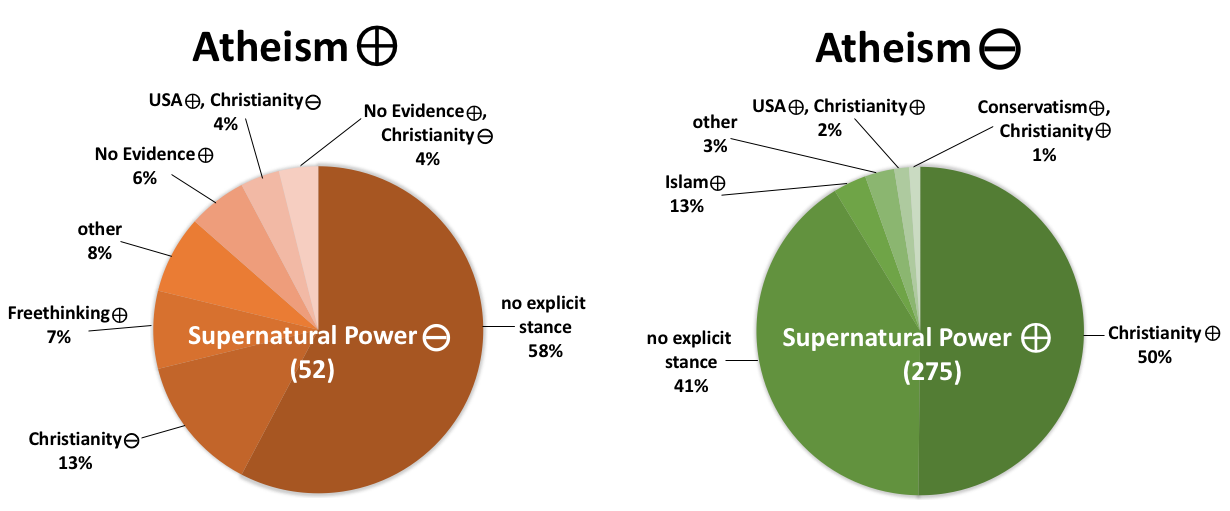
\includegraphics[width=0.9\textwidth]{figures/combinedPatterns_reduced.png}
   \caption{Most frequently used, explicit stances and the percentage shares to which they cooccur with other explicit stances}
  \label{fig:patterns_combined}
\end{figure*}

\subsection{Automatically Assigning Stances}
In order to investigate how well our model can be assigned automatically, we conduct classification experiments and compare with suitable baselines.
Based on how well the components are classifiable, we can derive how well the model is assignable as a whole.

We re-implement a state-of-the-art classifier \cite{StanceSemEval2016} using the DKPro TC framework\footnote{version 0.8.0} \cite{daxenberger2014dkpro} and leave the development of sophisticated classification models to future research.
For preprocessing, we rely on the DKPro Core framework\footnote{version 1.7.0} \cite{eckartdecastilho-gurevych:2014:OIAF4HLT} and apply a twitter-specific tokenizer \cite{gimpel2011part}.
In all experiments, we use ten-fold cross-validation and report micro averaged $F_1$.

\paragraph{Explicit Stances}

\begin{table}
\small
\centering
\begin{tabular}{lcc}
\toprule
\textbf{Target (\# instances)} & \textbf{Baseline}   & \textbf{SVM}    \\
\midrule
Supernatural Power (335)     & .53 & .78\\
Christianity (223)           & .69 & .79\\
Islam (43)                   & .94 & .95 \\
%\textit{Secularism (21)}    & \textit{.965} & \textit{.972} \\
%\textit{Conservative Movement (12)}  & \textit{.983} & \textit{.986}\\
%\textit{Religious Freedom (7)}    & \textit{.988} & \textit{.990}\\
%\textit{USA (28)}                   & \textit{.961}  & \textit{.964}\\
%\textit{No Evidence (10)}         & \textit{.986} & \textit{.987}\\
%\textit{Life After Death (9)}     & \textit{.987} & \textit{.987} \\
%\textit{Same-Sex Marriage (15)}    & \textit{.979} & \textit{.978}\\
%\textit{Freethinking (31)}         & \textit{.986} & \textit{.957}\\
\bottomrule
\end{tabular}
\caption{Explicit stance classification (only showing targets occurring in at least 5\% of all instances)}
\label{table:classificationExplicitStances}
\end{table}

As the result from the stance detection task in SemEval-2016 \cite{StanceSemEval2016} indicate, a support vector machine equipped with simple word and character n-gram features is the state of the art in automated stance prediction.
Table~\ref{table:classificationExplicitStances} shows the results of the state-of-the-art classifier and the majority class baseline for comparison.
The results indicate that the two most frequent targets can be classified with success, if one relates them to the majority class baseline.
We observe that each target has its own linguistic markers such as the use of Arabic terms if one is in favor of Islam. 
Therefore, we argue that these peculiarities can be targeted even better by specialized features.

The analysis in table~\ref{table:classificationExplicitStances} excludes targets that have a insufficient coverage (less than 5\% of all instances) to train a meaningful model.
A possibility to deal with this sparsity may be to incorporate unlabelled data such as demonstrated for traditional models by \newcite{habernal2015exploiting}.

\paragraph{Debate Stance}

\begin{table}[]
\small
\centering
\begin{tabular}{lc}
\toprule
Feature Set    & F$_1$ \\
\midrule
baseline       & .49            \\[5pt]
n-gram          & .66             \\
ngram + explicit stance$_{predicted}$ & .67            \\
ngram + explicit stance$_{oracle}$ &  .88      \\
explicit stance$_{predicted}$ & .65  \\
explicit stance$_{oracle}$ & .88  \\
\bottomrule         
\end{tabular}
\caption{Debate stance classification}
\label{table:classificationDebateStances}
\end{table}

Table~\ref{table:classificationDebateStances} shows the results obtained for automatically assigning the debate stance.
Besides the majority class baseline ($F_1=.49$), we use the same setup as for the explicit stances to train an n-gram based classifier and obtain an $F_1$ of $.66$.
In order to evaluate the usefulness of explicit stances for inferring the debate stance, we use the predictions from the previous experiment as features for a decision tree classifier (J48).
This stacked classifier performs on par ($.65$) with the n-gram based classifier.
It seems that the quality of predicting explicit stances is not yet good enough to improve over the state-of-the-art without incorporating general n-gram features.
To estimate the potential of explicit stance features for classifying the debate stance, we add an oracle condition to our experiments in which we assume that the classification of explicit stances is done correctly.
This classifier using only the manually annotated explicit stances yields an $F_1$ score of $.88$ showing that large improvements over the state of the art are possible if explicit stances can be more reliably classified.
We believe that this is indeed possible as explicit stances are always grounded in the text itself, while the debate stance might only be indirectly inferred.


\section{Remaining Problems}
The previously conducted experiments are only a first step towards argument mining that is robust against less elaborated and implicit arguments.
At the present time we identify four major lines of future work.  

\subsection{Advanced Machine Learning Techniques and Feature Engineering}
So far, we applied standard machine learning techniques ($SVM$ equipped with word n-grams) to the classification tasks.
At the moment we modelled the task as a document classification (i.e. the targets are classified independently).
Since we assume that there are strong dependencies between the targets, future experiments should implement a sequence classification by using e.g. $SVM_{HMM}$ of conditional random fields. 

As indicated by \newcite{habernal2015exploiting} and \newcite{mohammad2016stance} leveraging huge amounts of unlabelled data is beneficial for stance classification.
The idea behind this is to address the data sparsity with approaches such as bootstrapping or distant supervision.
In addition, the sparsity problem could be tackled by utilizing lexical semantic resources such as Wikipedia and semantic relatedness of words.
Consequently, we want to run experiments that implement these methods.

Moreover our model should profit from features that are tailored to certain explicit targets.
For instance, features that capture references passages by using regular expressions or text similarity measures towards the Bible should be beneficial for classifying the target \textit{Christianity}.

While the debate stance of an utterance is -- of course -- dependent on the current debate, models for classifying stance towards explicit targets should be domain more domain indepedent. 
Although this is an assumption that has to be proved, it is hard to imagine a domain in whichI love Jesus the utterance \textit{I love Jesus} does not express a favorization of \textit{Christianity}.
Consequently, it should be possible to create a collection of models for classifying explicit stances that could be applied to a new debate in the manner of a building block system.


\subsection{Selection of Explicit Targets}
In our model, choosing the right number and granularity of targets is crucial.
On the one hand, they have to be expressive enough to capture differences in nuanced argumentation.
On the other hand, they should not be too fine grained as this would result in very sparse distributions that cannot be handled by automated methods.
In our previous work \cite{wojatzki2016stanceBased}, we used a simple frequency approach that focussses on nouns and named entities only.
However, at the moment it is unclear how well the resulting set is able to describe the actually used explicit targets. 
Consequently, we want to examine this problem from three perspectives:
\begin{itemize}
  \item Gold Standards and Evaluation: Especially critical is to develop appropriate methods that allow to assess the performance of selection approaches. Therefore we need to create gold standard data and choose meaningful measures. We are currently looking for ideas to operationalize such data generation. 
  \item Theoretical Framework: We need a better theoretical understanding of how and what humans perceive as being explicitly expressed. One approach could be to examine the processes which are believed to enable humans to summarize Here we also want to gain a deeper understanding on how this relates to lexical priming effects -- the assumed basis of implicit argumentation.
  \item Modelling and Operationalizability: Ultimately, it comes to find better targets that approximate  the created gold data and align theoretical considerations. Therefore we plan to apply more advanced approaches from corpus linguistics such as $tf.idf$ or statistical topic modelling (e.g. $LDA$). It seems very promising to consider a clustering of synonyms or lexical substitutes of frequent nouns ($tf.idf$ selected nouns, etc.). With this goal in mind we already showed that lexical substitution can model ambiguity well \cite{wojatzki2016bundled}.
\end{itemize}

\subsection{Overall Model}
Insight form the previously conducted experiments suggests that our model can be improved in certain apects.
First, our model is adapted to texts that contain a high amount of implicit claims, but cannot express  the extent of implicitness.
Therefore for future work we want to make sure that the debate target is always contained in the set of explicit targets regardless of how frequent it is explicitly expressed.
Second, as the granularity of the explicit targets is still unclear, the best way may be to model copuld be to use multiple layers or explicit targets (increasingly implicit).
A question that arises here is whether the model should actually be grounded to the surface form of the utterances or rather to a more abstract representation such as the abstract meaning representation by \newcite{banarescu2012abstract}.
Of course, such an additional layer may also be a source of error.

Moreover, our current model is adapted to short utterances (i.e. tweets). 
Although our model allows more than one explicit targets per utterances, it is unclear if it is applicable for long documents.
This yields the question on whether our model should be sentence wide or a document-wide one.

\subsection{Application}
As described above we developed and tested our modle on a narrow domain and a limited amount of data.
However, the true value of our model will be seen only if it is applied to different domains and use-cases.

to gain more insight it would also be very interesting what happens if we apply schema to well formed text, formal texts (legal domain)
For this purpose, we are always interested in collaborations and interesting application areas for our model :)



% include your own bib file like this:
%\bibliographystyle{acl}
%\bibliography{acl2016}
\bibliography{acl2016}
\bibliographystyle{acl2016}


\end{document}
